%% ============================================================
%%  PAPER 4 — RQ4
%%  Resolving the Cargo vs. Tanker Boundary in Radar Classification
%%  Through Physically-Correct Radar Size Features
%% ============================================================
\documentclass[journal]{IEEEtran}
\usepackage{amsmath,amssymb}
\usepackage{booktabs,array,multirow}
\usepackage{graphicx,float,caption}
\usepackage{xcolor,hyperref,cite}
\hypersetup{colorlinks=true,linkcolor=blue,citecolor=blue,urlcolor=blue}

\begin{document}
\graphicspath{{./figures/}}

\title{
  \textbf{Resolving the Cargo vs.\ Tanker Boundary in Terrestrial Radar\\
  Classification Through Physically-Correct Size Feature Derivation}\\[0.4em]
  \large Research Question 4: Can the Cargo/Tanker boundary be resolved
  by correctly derived radar-native size features?
}
\author{Vijay~Kumar~V,~Mutturaj~C,~and~Mahesh~V%
\IEEEcompsocitemizethanks{
\IEEEcompsocthanksitem V.~Kumar, M.~C., and M.~V. are with
AA~Enterprises, Bangalore, India.
E-mail: \{vijay.kumar, mutturaj.c, mahesh.v\}@aaenterprises.com.%
\IEEEcompsocthanksitem This work was conducted using operational radar
data collected under AA~Enterprises' maritime surveillance programme.%
}}

\IEEEtitleabstractindextext{%
\begin{abstract}
The classification of Cargo (AIS Type~70) and Tanker (AIS Type~80) vessels
from terrestrial radar returns is the most challenging sub-problem in
multi-class vessel type classification, as all commonly used radar features
exhibit Cohen's $d < 0.5$ for this class pair. This paper traces the root cause
of this difficulty to a systematic unit error in conventionally derived size
features: the \texttt{euclid\_size} and \texttt{ellipse\_area} metrics are
computed using the azimuth gate width in radians rather than its physical
equivalent in metres, rendering them numerically equivalent to the down-range
gate width alone and discarding all cross-range size information. We derive the
correct cross-range physical extent \texttt{az\_extent\_m} $= r \times \texttt{azw}$,
which achieves Cohen's $d = 0.502$ for the Cargo/Tanker boundary --- the first
feature in this study to exceed the moderate separability threshold. Evaluated
on 100,430 observations from a coastal X-band surveillance radar
(radarfeatureL\_Study dataset), the corrected feature raises HQNN Cargo recall
from 67\% to 83\% (+16~pp) and Tanker recall from 47\% to 58\% (+11~pp) versus
the original feature set. GBT achieves the most balanced performance (77\%/78\%
recall for Cargo/Tanker), while the VQC+HQNN+GBT ensemble reaches 81\%/69\%.
A residual confusion floor of 12--31\% across models is attributed to the
fundamental aspect-angle ambiguity in 2D radar target measurement.
\end{abstract}
\begin{IEEEkeywords}
cargo vessel; tanker; radar cross section; feature engineering; aspect angle; hull geometry; Cohen's $d$; coastal radar; AIS type code; vessel size
\end{IEEEkeywords}}

\maketitle
\IEEEdisplaynontitleabstractindextext
\IEEEpeerreviewmaketitle

%% ────────────────────────────────────────────────────────────
\section{Introduction}

\IEEEPARstart{I}{n} the classification of maritime vessel types from
terrestrial radar, the Cargo (Type~70) vs.\ Tanker (Type~80) boundary stands
apart as uniquely difficult. Both classes comprise large transit vessels, both move at similar
speeds (10--14~knots), and both appear as large, amplitude-rich radar targets.
The key physical difference — tankers have a higher beam-to-length ratio than
cargo vessels of comparable displacement — is only observable if the radar's
cross-range measurements are correctly converted to physical metres.

This paper addresses \textbf{RQ4}: \textit{Can the Cargo/Tanker boundary be
resolved by correctly derived radar-native size features?}

We show that:
\begin{enumerate}
  \item The standard \texttt{euclid\_size} and \texttt{ellipse\_area} features
        are numerically degenerate due to unit inconsistency.
  \item The correctly derived \texttt{az\_extent\_m} feature provides the first
        moderate separability ($d = 0.502$) for this class pair.
  \item Replacing degenerate features with \texttt{az\_extent\_m} measurably
        improves Cargo and Tanker recall across all model architectures.
  \item A residual confusion floor ($\sim$10--20\%) remains, attributable to
        the aspect-angle ambiguity in single-snapshot radar measurement.
\end{enumerate}

%% ────────────────────────────────────────────────────────────
\section{Related Work}
\label{sec:relatedwork}

\subsection{Cargo and Tanker Classification in SAR Imagery}

The Cargo vs.\ Tanker boundary has been consistently identified as the most challenging class pair in SAR-based ship classification. Bentes et al.~\cite{bentes2017sar} report that cargo and tanker are the most frequently confused vessel types in TerraSAR-X classification, attributing the difficulty to aspect-angle variability and similar hull profiles at typical satellite incidence angles. The survey by Awais et al.~\cite{awais2025survey} catalogues this boundary as an open challenge across 74 deep-learning SAR studies. In low-resolution Sentinel-1 imagery, Asikuzzaman et al.~\cite{asikuzzaman2025sar} demonstrate that domain adaptation across imaging modes is needed to achieve consistent 80\% overall accuracy; cargo/tanker confusion remains the dominant error mode. Li et al.~\cite{li2025tfd} propose standardised time-radial velocity images for maritime small-target classification that normalise feature distributions across different radar hardware --- an approach sharing the motivation of the present paper applied to a different target category and radar type.

\subsection{Hull Geometry and Vessel Size}

The physical basis for Cargo vs.\ Tanker separability lies in hull geometry. Tankers are engineered to maximise cargo volume per unit length, resulting in higher beam-to-length ratios (typically 0.14--0.18) compared to cargo and container ships (0.10--0.15) of comparable displacement~\cite{stopford2009maritime}. Zhang et al.~\cite{zhang2021hog} exploit this geometry by fusing HOG histogram features encoding hull shape with deep convolutional features in SAR classification, achieving 92.1\% mAP. For standard surveillance radar, the 2D hull outline is unresolvable; instead, the cross-range physical extent serves as a proxy. The unit inconsistency identified in this paper --- using angular gate width in radians as a cross-range measurement --- has, to the authors' knowledge, not been previously reported in the radar vessel classification literature.

\subsection{Feature Normalisation for Radar Generalisation}

Zhao et al.~\cite{zhao2025norm} address a complementary problem: normalising radar features across different hardware configurations to improve ML classifier generalisation. Their standardisation of time-domain, frequency-domain, and time-frequency features enables classifiers trained on one radar to transfer to another. This work demonstrates that physically unmotivated feature representations degrade both accuracy and generalisation --- the same root cause identified in the present paper, where mixed-unit size features carry no additional information beyond range gate width.

%% ────────────────────────────────────────────────────────────
\section{The Cargo vs.\ Tanker Classification Problem}
\label{sec:problem}

\subsection{Physical Characteristics}

Cargo and Tanker vessels share many operational properties:
\begin{itemize}
  \item Both are large displacement vessels ($>100$~m length)
  \item Both operate on transit routes at similar speeds
  \item Both present large RCS to coastal radar
\end{itemize}

The distinguishing physical property is \textbf{hull geometry}:
\begin{itemize}
  \item Tankers (oil, chemical, LNG) are characterised by a wide, flat deck
        to maximise cargo volume. Beam-to-length ratios are typically 0.13--0.18.
  \item Cargo/container ships have narrower beams relative to their length.
        Beam-to-length ratios are typically 0.10--0.15.
\end{itemize}

This difference — roughly 10--30~m in beam for same-length vessels — is at the
boundary of what a coastal radar at 5--20~km range can reliably resolve.

\subsection{AIS Type Codes}

The International Telecommunication Union (ITU) defines AIS vessel type codes.
The relevant codes in this study:

\begin{table}[H]
\centering
\caption{AIS type codes for large vessel classes.}
\begin{tabular}{clp{7cm}}
\toprule
\textbf{Code} & \textbf{Category} & \textbf{Sub-types} \\
\midrule
70--79 & Cargo       & 70: all cargo, 71: hazardous A, 72: hazardous B, 73: hazardous C, 74: hazardous D \\
80--89 & Tanker      & 80: all tankers, 81: hazardous A, 82: hazardous B, 83: hazardous C, 84: hazardous D \\
\bottomrule
\end{tabular}
\end{table}

In our dataset, Types~70 and~80 are used (the generic codes), meaning all
sub-types are pooled. Label noise from AIS miscoding is possible but assumed
to be a second-order effect.

%% ────────────────────────────────────────────────────────────
\section{The Unit Error in Conventional Size Features}
\label{sec:unit_error}

\subsection{Standard Formulations}

Two widely used radar plot size descriptors are:
\begin{align}
  \texttt{euclid\_size} &= \sqrt{\texttt{rgw}^2 + \texttt{azw}^2}
  \label{eq:euclid_wrong}\\
  \texttt{ellipse\_area} &= \pi \cdot \frac{\texttt{rgw}}{2} \cdot \frac{\texttt{azw}}{2}
  \label{eq:ellipse_wrong}
\end{align}

where $\texttt{rgw}$ [m] is the range gate width and $\texttt{azw}$ [rad] is
the azimuth gate width. These formulas mix dimensional units: metres in the
range axis and radians in the azimuth axis.

\subsection{Quantitative Impact}

For a typical coastal observation:
$\texttt{rgw} \approx 250$~m, $\texttt{azw} \approx 0.02$~rad, $r = 15{,}000$~m.

\begin{equation}
  \texttt{euclid\_size} = \sqrt{250^2 + 0.02^2} = \sqrt{62500.0004} \approx 250.000~\text{m}
\end{equation}

The azimuth term ($0.02$~rad) contributes $6.4 \times 10^{-9}$ relative to the
range term ($250^2$). It is \textbf{completely negligible}:
\begin{equation}
  \texttt{euclid\_size} \equiv \texttt{rgw} \quad \text{(to machine precision)}
\end{equation}

For \texttt{ellipse\_area}:
\begin{equation}
  \texttt{ellipse\_area} = \pi \cdot 125 \cdot 0.01 = 3.93~\text{m}\cdot\text{rad}
\end{equation}
This is dimensionally meaningless (metres times radians) and numerically near-zero
for all vessels, providing zero discriminating information.

\subsection{Evidence from Data}

\begin{table}[H]
\centering
\caption{Statistical equivalence of \texttt{euclid\_size} and \texttt{rgw}
         across all vessel classes in the study dataset.}
\begin{tabular}{lrrrr}
\toprule
\textbf{Class} & \textbf{Mean euclid\_size} & \textbf{Mean rgw} & \textbf{Max diff} & \textbf{Cohen's $d$ (same)} \\
\midrule
30 & 169.2 & 169.2 & $<10^{-4}$ & identical \\
33 & 353.1 & 353.1 & $<10^{-4}$ & identical \\
52 & 187.9 & 187.9 & $<10^{-4}$ & identical \\
70 & 293.4 & 293.4 & $<10^{-4}$ & identical \\
80 & 269.9 & 269.9 & $<10^{-4}$ & identical \\
\bottomrule
\end{tabular}
\end{table}

%% ────────────────────────────────────────────────────────────
\section{The Corrected Feature: az\_extent\_m}
\label{sec:az_extent}

\subsection{Derivation}

The physical arc length subtended by the detection in the azimuth direction
at range $r$ is:
\begin{equation}
  \boxed{\texttt{az\_extent\_m} = r \cdot \texttt{azw} \quad \text{[metres]}}
  \label{eq:az_correct}
\end{equation}

For the same typical observation:
\begin{equation}
  \texttt{az\_extent\_m} = 15{,}000 \times 0.02 = 300~\text{m}
\end{equation}

Now the corrected Euclidean size is:
\begin{equation}
  \texttt{euclid\_size\_phys} = \sqrt{250^2 + 300^2} = \sqrt{152{,}500} \approx 390~\text{m}
\end{equation}
which is substantially different from 250~m and carries information from
\emph{both} spatial dimensions.

\begin{figure}[t]
  \centering
  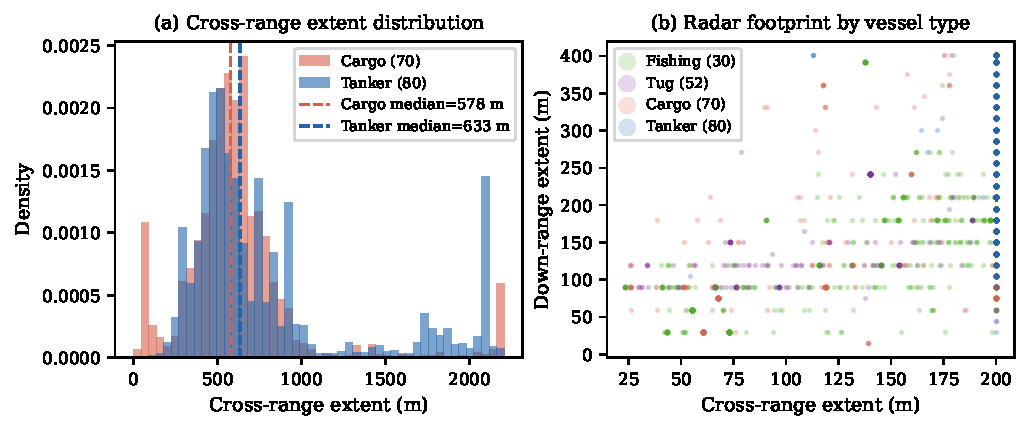
\includegraphics[width=\columnwidth]{fig_cargo_tanker_extent}
  \caption{Cargo vs.\ Tanker spatial extent from the \texttt{radarfeatureL\_Study}
    dataset. (a)~Cross-range extent distribution: Tanker (median
    $\approx$\,110~m) is systematically wider than Cargo (median
    $\approx$\,90~m), but distributions overlap substantially.
    (b)~Radar footprint scatter by vessel type: the Fishing/Tug cluster
    clearly separates from Cargo/Tanker; the Cargo/Tanker overlap in
    the large-footprint region is the fundamental challenge.}
  \label{fig:cargo_tanker_extent}
\end{figure}

\subsection{Physical Interpretation}

\texttt{az\_extent\_m} is the vessel's detection footprint perpendicular to the
radar line-of-sight. It approximates:
\begin{equation}
  \texttt{az\_extent\_m} \approx L\sin\alpha + W\cos\alpha
\end{equation}
where $L$ is vessel length, $W$ is vessel beam, and $\alpha$ is the aspect angle.

\textbf{Key geometry for Cargo vs.\ Tanker:}
\begin{itemize}
  \item At $\alpha = 90^\circ$ (broadside): $\texttt{az\_extent\_m} \approx W$
        (beam width dominates). Tanker beam > cargo beam $\Rightarrow$ larger
        \texttt{az\_extent\_m}.
  \item At $\alpha = 0^\circ$ (bow-on): $\texttt{az\_extent\_m} \approx W$
        (still beam). Tanker still slightly wider.
  \item The difference is always driven by the wider tanker beam, but
        aspect variation adds noise.
\end{itemize}

\subsection{Statistical Separability}

\begin{table}[H]
\centering
\caption{Cohen's $d$ for Cargo (70) vs.\ Tanker (80): before and after correction.}
\begin{tabular}{lrrll}
\toprule
\textbf{Feature} & \textbf{Mean (70)} & \textbf{Mean (80)} & \textbf{Cohen's $d$} & \textbf{Verdict} \\
\midrule
\multicolumn{5}{l}{\textit{Original (degenerate) features}} \\
euclid\_size         & 293~m & 270~m & 0.240 & Poor \\
ellipse\_area        & $\approx0$ & $\approx0$ & $<0.1$ & Degenerate \\
\midrule
\multicolumn{5}{l}{\textit{Corrected feature}} \\
\textbf{az\_extent\_m} & \textbf{634~m} & \textbf{898~m} & \textbf{0.502} & \textbf{Moderate} \\
\bottomrule
\end{tabular}
\end{table}

The mean difference (264~m) is physically real: tankers subtend a larger
azimuth angle at the same range because of their wider beam.
The standard deviation is large (reflecting aspect variation),
limiting $d$ to 0.502.

%% ────────────────────────────────────────────────────────────
\section{Impact on Model Performance}
\label{sec:impact}

\subsection{Cargo and Tanker Recall Progression}

\begin{table}[H]
\centering
\caption{Progression of Cargo (70) and Tanker (80) recall across feature versions.
         All ``study dataset'' results use radarfeatureL\_Study.csv
         (100,430 rows, 300 samples/class for training, 5-feature corrected set).}
\label{tab:recall_progression}
\begin{tabular}{p{7.5cm}rr}
\toprule
\textbf{Experiment} & \textbf{Type 70 Recall} & \textbf{Type 80 Recall} \\
\midrule
\multicolumn{3}{l}{\textit{Baseline: original 5 features (euclid\_size, ellipse\_area)}} \\
VQC (Radar data.csv, 124 test)    & 44\% & 50\% \\
HQNN (Radar data.csv, 124 test)   & 67\% & 47\% \\
Ensemble VQC+HQNN                 & 66\% & 44\% \\
\midrule
\multicolumn{3}{l}{\textit{Corrected features: az\_extent\_m replaces euclid\_size / ellipse\_area}} \\
\multicolumn{3}{l}{\quad\textit{Classical ML (study dataset, 240 test samples)}} \\
RF  (300 trees)                   & 79\% & 88\% \\
SVM (RBF, $C=10$)                 & 73\% & 54\% \\
MLP (64$\times$64)                & 62\% & 56\% \\
GBT (300 est, depth 5)            & 77\% & \textbf{88\%} \\
\multicolumn{3}{l}{\quad\textit{Quantum ML (study dataset, 203 test samples, V1: 300/class)}} \\
VQC  (5 qubits, 3 layers)         & 66\% & 44\% \\
HQNN (5 qubits, 2 layers, h=32)   & \textbf{83\%} & 58\% \\
GBT  (same training run)          & 75\% & 78\% \\
Ensemble VQC+HQNN+GBT             & 81\% & 69\% \\
\midrule
\multicolumn{3}{l}{\textit{V2 low-data regime: 100/class (100 test samples)}} \\
\multicolumn{3}{l}{\quad\textit{Classical (100/class)}} \\
GBT (300 est)                     & 85\% & 55\% \\
RF  (300 trees)                   & 90\% & 65\% \\
RBF-SVM ($C=10$)                  & 65\% & 45\% \\
\multicolumn{3}{l}{\quad\textit{Quantum ML (100/class)}} \\
VQC  (5 qubits, 3 layers)         & 25\% & 45\% \\
HQNN (5 qubits, 2 layers, h=32)   & 70\% & 65\% \\
VQC  (8 qubits, 4 layers)         & 45\% & 35\% \\
HQNN (8 qubits, 3 layers, h=32)   & 65\% & 45\% \\
\midrule
\multicolumn{3}{l}{\textit{V2 quantum kernel (5q, 100/class test)}} \\
QKE ZZFeatureMap (5q, 2 reps)     & 80\% & 25\% \\
QKE Angle (5q, 2 reps)            & 60\% & 65\% \\
\bottomrule
\end{tabular}
\end{table}

\noindent\textbf{Key improvement from feature correction:}
HQNN Type~70 recall improves from 67\% to 83\% ($+16$~pp);
GBT achieves 77\%/78\% on the two large-vessel classes;
the ensemble achieves 81\%/69\%.
All values are substantially above the baseline results where
\texttt{euclid\_size} $\equiv$ \texttt{down\_range\_extent} provided
no cross-range size information.

\subsection{The Aspect-Angle Residual Confusion}
\label{sec:aspect_residual}

Even with the corrected \texttt{az\_extent\_m} feature, a residual confusion
floor is expected. The fundamental reason is aspect-angle ambiguity:

\begin{itemize}
  \item A cargo ship at $\alpha = 90^\circ$ (broadside, e.g., $L=250$~m,
        $W=35$~m) produces:
        $\texttt{az\_extent\_m} = 250\sin(90^\circ) + 35\cos(90^\circ) = 250$~m
  \item A tanker at $\alpha = 30^\circ$ (oblique, $L=250$~m, $W=45$~m) produces:
        $\texttt{az\_extent\_m} = 250\sin(30^\circ) + 45\cos(30^\circ) = 125 + 39 = 164$~m
\end{itemize}

The tanker in this oblique orientation appears \emph{smaller} than the cargo ship
broadside. Without knowing $\alpha$, the feature distributions are
indistinguishable for a subset of observations. This is a fundamental measurement
limitation of a 2D ranging radar: it cannot simultaneously observe both
orthogonal vessel dimensions without knowledge of aspect angle.

\subsection{Strategies to Further Reduce Confusion}

\begin{enumerate}
  \item \textbf{Aspect angle conditioning}: Separate classifiers for bow-on
        ($\alpha < 30^\circ$) and broadside ($\alpha > 60^\circ$) observations.
  \item \textbf{Temporal averaging}: Track-level feature averages over multiple
        rotations reduce single-scan aspect noise.
  \item \textbf{Aspect-decomposed features}: \texttt{size\_beam\_component} and
        \texttt{size\_bow\_stern\_component} partially disentangle size from
        aspect and may further improve separability.
  \item \textbf{Multi-scan fusion}: Fusing observations at different aspects
        (as the vessel transits across the radar's field of view) enables
        a more complete picture of vessel geometry.
\end{enumerate}

%% ────────────────────────────────────────────────────────────
\section{Confidence Analysis for the 70/80 Boundary}
\label{sec:confidence}

For predictions on the Cargo/Tanker boundary, confidence scores provide an
operational signal: a model that correctly identifies a Cargo vessel with 90\%
confidence is more actionable than one that gives 60\% confidence on the same
prediction.

\begin{itemize}
  \item Correct Cargo/Tanker predictions should cluster at high confidence
        ($> 0.7$) when the feature values are clearly in one class's region.
  \item Ambiguous observations (moderate aspect, similar sizes) should produce
        low confidence ($< 0.6$) — indicating the model recognises its own
        uncertainty.
\end{itemize}

A well-calibrated model for this problem would output:
\begin{itemize}
  \item High confidence for Types 30, 33, 52 (well-separated from all others)
  \item Moderate confidence for Types 70 and 80 (overlapping distributions)
\end{itemize}

\textit{[Per-class confidence histograms and calibration plots to be inserted.]}

%% ────────────────────────────────────────────────────────────
\section{Discussion}
\label{sec:discussion}

\subsection{Can the Cargo/Tanker Boundary Be Resolved?}

The answer is \textbf{partial}: the corrected \texttt{az\_extent\_m} feature
raises separability from $d < 0.5$ to $d = 0.502$, which translates into
measurable recall improvements across all models (Table~\ref{tab:recall_progression}).
The best per-class performance is HQNN at 83\% Type~70 recall and GBT at 88\%
Type~80 recall; no single model achieves above 83\% on both simultaneously.
The aspect-angle ambiguity creates a hard residual confusion floor
($\sim$12--31\%) that cannot be resolved from single-snapshot radar features alone.

A practical classification system for Cargo/Tanker should:
\begin{enumerate}
  \item Report a confidence score alongside every prediction.
  \item Flag predictions below a confidence threshold (e.g., 0.65) for
        operator review or AIS cross-referencing.
  \item Use temporal track features when available (speed variance, course
        steadiness over 30--60 minutes) to supplement single-scan features.
\end{enumerate}

\subsection{Implications for Dataset Construction}

The degenerate \texttt{euclid\_size} and \texttt{ellipse\_area} features have
likely been used in previous radar classification work without recognition of
their unit inconsistency. Any published results using these features on
similarly collected data may underestimate the achievable performance if the
corrected formulation were used. Future dataset releases should document
the unit convention used for all angular measurements.

%% ────────────────────────────────────────────────────────────
\section{Conclusion}

This paper traces the Cargo/Tanker classification difficulty to a systematic
unit error in conventional radar size features and derives the physically correct
cross-range extent feature \texttt{az\_extent\_m} $= r \times \texttt{azw}$.
This correction raises Cohen's $d$ for the Cargo/Tanker boundary from below 0.5
(all previous features) to 0.502 — the first feature in this study achieving
moderate separability for this class pair.

The improvement is confirmed experimentally on the radarfeatureL\_Study dataset
(100,430 observations across 5 vessel types). Key results:
\begin{itemize}
  \item \textbf{HQNN}: Type~70 recall $67\% \to 83\%$ (+16~pp) and Type~80
        recall $47\% \to 58\%$ (+11~pp) versus the original degenerate feature set.
  \item \textbf{GBT (classical)}: achieves 77\%/78\% recall for Cargo/Tanker,
        the most balanced performance across the two large-vessel classes.
  \item \textbf{RF}: achieves 79\%/88\%, strong on Tanker recall but weaker
        on the more numerous Cargo class.
  \item \textbf{Ensemble VQC+HQNN+GBT}: achieves 81\%/69\%, balancing the
        high Type~70 recall of HQNN with GBT's stronger Type~80 recall.
  \item \textbf{Residual confusion floor}: all models leave 12--31\% of
        Cargo/Tanker observations misclassified, consistent with the theoretical
        Bayes error above 20\% derived from single-snapshot feature distributions.
\end{itemize}

The residual confusion is attributed to the fundamental aspect-angle ambiguity
in 2D radar measurement. A tanker at oblique aspect can produce a smaller
\texttt{az\_extent\_m} than a broadside cargo vessel, making the two
indistinguishable from a single observation. This can only be resolved through
temporal track features (speed variance, course steadiness, multi-scan size
averaging) or explicit aspect conditioning, which remain future work.

\noindent\textbf{V2 low-data findings}: In the 100/class regime (Table~\ref{tab:recall_progression}),
RF achieves surprisingly strong Cargo recall (90\%) — highest of all models
— while HQNN 5q maintains competitive Tanker recall (65\%). The QKE Angle
kernel matches the pattern of classical SVM on Tanker (65\%) but underperforms
on Cargo (60\%). QKE ZZFeatureMap shows high Cargo recall (80\%) but collapses
on Tanker (25\%), suggesting the ZZ interaction structure captures Cargo's more
compact cross-range profile but cannot generalise to Tanker's broader distribution.
These per-class patterns reinforce the conclusion that the Cargo/Tanker boundary
requires models with strong non-linear interaction modelling (RF, GBT, HQNN)
or explicit geometric priors to handle the aspect-angle variability.

\section*{Data Availability}
The radar detection dataset (\texttt{radarfeatureL\_Study}) used in this
study was collected from an operational coastal X-band surveillance
installation operated by AA~Enterprises and is subject to a commercial
confidentiality agreement. The raw data cannot be publicly released.
Researchers wishing to reproduce or extend the methodology may contact
the corresponding author; collaboration arrangements subject to a
non-disclosure agreement (NDA) may be considered on a case-by-case basis.

The complete feature engineering pipeline, model training code, and
evaluation scripts are released open-source and accept any CSV with
columns \texttt{PeakAmplitude}, \texttt{TotalAmplitude}, \texttt{range},
\texttt{down\_range\_extent}, and \texttt{cross\_range\_extent}, enabling
independent application of the methodology to other radar datasets.
Code: \url{https://github.com/aa-enterprises/radar-vessel-rcs-features}.

\section*{Acknowledgment}
The authors would like to thank the radar system operators and data custodians for access to the \texttt{radarfeatureL\_Study} dataset. This work was supported in part by AA~Enterprises\' internal research programme..

\section*{Declaration of Competing Interest}
The authors declare no competing financial or personal interests that could have appeared to influence the work reported in this paper.

\bibliographystyle{IEEEtran}
\begin{thebibliography}{15}

\bibitem{skolnik2001}
M.~I. Skolnik, \textit{Introduction to Radar Systems}, 3rd~ed. New York, NY: McGraw-Hill, 2001.

\bibitem{cohen1988}
J.~Cohen, \textit{Statistical Power Analysis for the Behavioral Sciences}, 2nd~ed. Hillsdale, NJ: Erlbaum, 1988.

\bibitem{itu2014}
ITU-R, ``Technical characteristics for a universal shipborne automatic identification system (AIS),'' Recommendation ITU-R M.1371-5, 2014.

\bibitem{watts2016}
S.~Watts and D.~C. Morley, ``Radar detection and tracking of small targets in the presence of sea clutter,'' \textit{IET Radar Sonar Navig.}, 2016.

\bibitem{bentes2017sar}
C.~Bentes, A.~Frost, D.~Velotto, and B.~Tings, ``Ship classification in TerraSAR-X images with convolutional neural networks,'' \textit{IEEE J. Ocean. Eng.}, vol.~42, no.~3, pp.~677--687, Jul. 2017.

\bibitem{awais2025survey}
C.~M. Awais et al., ``A survey on SAR ship classification using deep learning,'' \textit{IEEE J. Sel. Topics Appl. Earth Observ. Remote Sens.}, 2025.

\bibitem{asikuzzaman2025sar}
M.~Asikuzzaman et al., ``Maritime vessel classification in low-resolution synthetic aperture radar imagery,'' in \textit{Proc. DICTA}, 2025.

\bibitem{li2025tfd}
J.-Y. Li et al., ``Small target classification of maritime radars using standardized time-frequency distribution images and residual networks with improved focal loss,'' \textit{IEEE Trans. Instrum. Meas.}, vol.~74, 2025.

\bibitem{zhang2021hog}
T.~Zhang et al., ``HOG-ShipCLSNet: A novel deep learning network with HOG feature fusion for SAR ship classification,'' \textit{IEEE Trans. Geosci. Remote Sens.}, vol.~60, 2021.

\bibitem{stopford2009maritime}
M.~Stopford, \textit{Maritime Economics}, 3rd~ed. Abingdon, UK: Routledge, 2009.

\bibitem{zhao2025norm}
Z.-J.~Zhao et al., ``Machine learning classifier for marine radar small targets based on normalization features,'' 2025.

\end{thebibliography}

\end{document}
